% Graphical abstract (Elsevier: 13 x 5 cm, readable at reduced size) -- TikZ source; also provided as Graphical_Abstract.drawio
\documentclass[tikz,border=2pt]{standalone}
\usepackage{amsmath}\usepackage{helvet}\renewcommand{\familydefault}{\sfdefault}
\usetikzlibrary{positioning,arrows.meta,calc}
% Document information of the PDF (Author = Thu Nguyen); see Scripts/set_figure_metadata.py
\pdfinfo{/Author (Thu Nguyen) /Title (Graphical abstract)}
\begin{document}
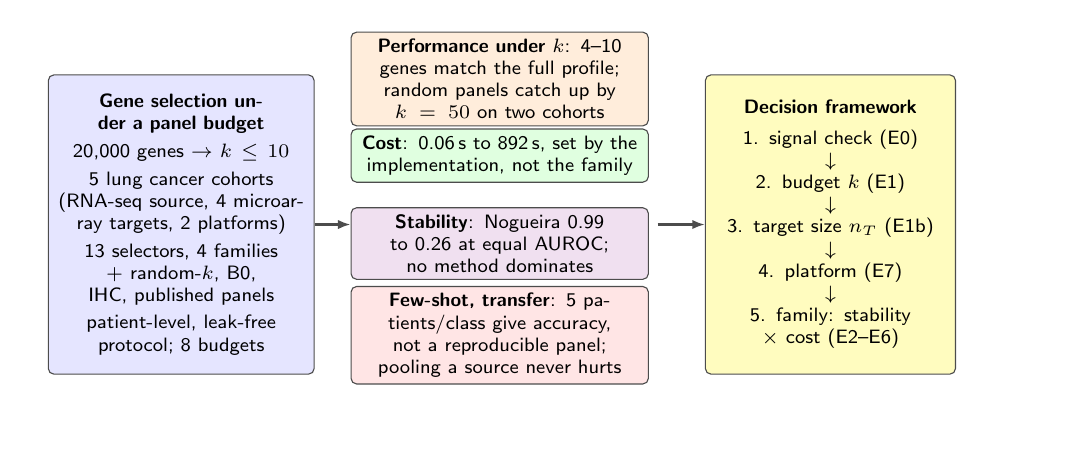
\begin{tikzpicture}[x=1cm,y=1cm,
  b/.style={draw=black!70, rounded corners=2pt, align=center, inner sep=2.5pt, font=\scriptsize},
  arr/.style={-{Latex[length=1.6mm]}, thick, black!70}]
\useasboundingbox (0,0) rectangle (13,5);
% left: setting
\node[b, fill=blue!10, text width=32mm, minimum height=38mm] at (1.95,2.5) (in) {\textbf{Gene selection under a panel budget}\\[2pt]20,000 genes $\to$ $k \le 10$\\[2pt]5 lung cancer cohorts\\(RNA-seq source, 4 microarray targets, 2 platforms)\\[2pt]13 selectors, 4 families\\$+$ random-$k$, B0, IHC, published panels\\[2pt]patient-level, leak-free protocol; 8 budgets};
% middle: four axes
\node[b, fill=orange!14, text width=36mm, anchor=north west] at (4.1,4.95) (a1) {\textbf{Performance under $k$}: 4--10 genes match the full profile; random panels catch up by $k = 50$ on two cohorts};
\node[b, fill=green!12, text width=36mm, anchor=north west] at (4.1,3.72) (a2) {\textbf{Cost}: 0.06\,s to 892\,s, set by the implementation, not the family};
\node[b, fill=violet!12, text width=36mm, anchor=north west] at (4.1,2.72) (a3) {\textbf{Stability}: Nogueira 0.99 to 0.26 at equal AUROC; no method dominates};
\node[b, fill=red!10, text width=36mm, anchor=north west] at (4.1,1.72) (a4) {\textbf{Few-shot, transfer}: 5 patients/class give accuracy, not a reproducible panel; pooling a source never hurts};
% right: framework
\node[b, fill=yellow!25, text width=30mm, minimum height=38mm, anchor=west] at (8.6,2.5) (out) {\textbf{Decision framework}\\[3pt]1. signal check (E0)\\$\downarrow$\\2. budget $k$ (E1)\\$\downarrow$\\3. target size $n_T$ (E1b)\\$\downarrow$\\4. platform (E7)\\$\downarrow$\\5. family: stability $\times$ cost (E2--E6)};
\draw[arr] (in.east) -- (4.1,2.5);
\draw[arr] (8.0,2.5) -- (out.west);
\end{tikzpicture}
\end{document}
